
\documentclass[conference]{IEEEtran}
\IEEEoverridecommandlockouts

\usepackage{cite}
\usepackage{amsmath,amssymb,amsfonts}
\usepackage{graphicx}
\usepackage{textcomp}
\usepackage{xcolor}
\usepackage{hyperref}
\usepackage{etoolbox}
\usepackage[utf8]{inputenc}

\def\BibTeX{{\rm B\kern-.05em{\sc i\kern-.025em b}\kern-.08em
    T\kern-.1667em\lower.7ex\hbox{E}\kern-.125emX}} 

\begin{document}

\title{\textbf{Assignment 2: The Raven Test \\ \LARGE{In Search for Group Differences}}\\
\vspace{10pt}
\Large Data Mining, University of Aveiro \\ 2019
}

\author{\IEEEauthorblockN{Filipe Pires, 85122}
\IEEEauthorblockA{\textit{DETI, MSc. Informatics Engineering}}
\and
\IEEEauthorblockN{João Alegria, 85048}
\IEEEauthorblockA{\textit{DETI, MSc. Informatics Engineering}}

}

\makeatletter
\patchcmd{\@maketitle}
{\addvspace{0.5\baselineskip}\egroup}
{\addvspace{-1\baselineskip}\egroup}
{}
{}
\makeatother

\maketitle

\begin{abstract}
...
\end{abstract} 

\begin{IEEEkeywords}
...
\end{IEEEkeywords}

\section{Introduction}

Lorem ipsum ...

\section{Dataset \& Feature Extraction}

Lorem ipsum ...

\section{Data Quality \& Normalization}
In relation to the dataset and the quality of the information present on it, through analysis of Table \ref{fig:feature}, which is the visual representation of the correlation of every possible pair of features, being the diagonal the pair composed of the feature with itself and is represented with a histogram that describe the value distribution inside that given feature, the remaining pairs are represented with scatter plots, we can take some important conclusions. The first one, which was already expected is that there was some outliers that needed to be taken care of, the second conclusion that's more important for this study is the fact that the data in all pairs of features doesn't appear to be separable, i.e., since there is two classes, the \textit{DEI} class and the \textit{ESEC} class there should be something resembling two groups, one for each class. That doesn't happen since in most cases we are presented with a uniform distributions, gaussian distributions or simply the grouping of all data in a unique central point. 

After familiarizing better with the data and understanding it better, it was needed to process it in a way that the models that we intend to apply have the best change of finding the distinguishing factors. For that we needed to remove the already mentioned outliers and normalize the data. We started by doing the mentioned normalization, which consisted in applying the \textit{ZSCORE} algorithm to each feature, which follows the Formula \ref{zscore} and already centers the data. Following this we also removed any data entry that contained a \textit{Null} values, since that would cause problems to the models' processing. Finally we removed the still existing outliers applying the Expression \ref{outliers}.

\begin{equation}\label{zscore}
    z_{i} = \frac{x_{i} - \mu}{\delta}
\end{equation}

\begin{equation}\label{outliers}
    |x_{i}-\mu| < 3\times\delta
\end{equation}

\section{Classifiers}
In this section we will present and give a brief summary of all the machine learning models used in this study.

\subsection{Support Vector Machine}
Commonly denoted as SVM, this supervised machine learning model with the supplied training set, by mapping the several data entries in the a multidimensional space in a way that the the widest possible gap exist between the data of each class. Based in that gap a model is created and a decision rule defined that when feed new data tries to assign a class to that entry by using the decision rule already mentioned.

\subsection{MultiLayer Perceptron}
This class of feedforward artificial neural network is another supervised machine learning model. MLP is sometimes strictly refers to networks composed of multiple layers of perceptrons. Perceptron is also a supervised learning algorithm capable of doing binary classifications according to a linear predictor function. The power of the MLP is the junction of several of those perceptrons that individually don't have the a good performance, but the combine performance can reach significant values.

This junction normally follows a standard architecture divided in layers, firstly a input layer, followed by one or more hidden layers and an output layer. The input and the output layers are the ones that interact with the exterior, being the first, as the name indicates teh one where the data should be injected at and the second where the result will be presented. The hidden layers is where the main learning occurs and where the most amount of fine-tunning is applied. In this entire architecture the number of layers and the number of neurons(singular cell inside a layer) can be tunning to improve the model performance.

\subsection{Decision Tree}
As the name suggests, this model uses a tree like structure to support the data classification decision. The construction of this auxiliary structure is quite simple and straightforward, consisting in assigning a condition to each new branch, causing that the structure will converge with having only one class in leaf nodes, defining the conditions required to identify the existing classes. 

\subsection{Random Forest}

\subsection{K Nearest Neighbors}

\section{Parameters Variation}

Lorem ipsum ...

\section{Results Discussion}

Lorem ipsum ...

\section{Conclusions \& Future Work}

Lorem ipsum ...

% \begin{itemize}
% \item Lorem ipsum ...
% \end{itemize}

% \begin{equation}
% a+b=\gamma\label{eq}
% \end{equation}

% ... \eqref{eq} ...

% ... Fig.~\ref{fig} ...

% \begin{table}[htbp]
% \caption{Table Type Styles}
% \begin{center}
% \begin{tabular}{|c|c|c|c|}
% \hline
% \textbf{Table}&\multicolumn{3}{|c|}{\textbf{Table Column Head}} \\
% \cline{2-4} 
% \textbf{Head} & \textbf{\textit{Table column subhead}}& \textbf{\textit{Subhead}}& \textbf{\textit{Subhead}} \\
% \hline
% copy& More table copy$^{\mathrm{a}}$& &  \\
% \hline
% \multicolumn{4}{l}{$^{\mathrm{a}}$Sample of a Table footnote.}
% \end{tabular}
% \label{tab1}
% \end{center}
% \end{table}

% \begin{figure}[h!]
% \centering
% \includegraphics[width=0.95\linewidth]{../img/screenshots/screenshot_map.png}
% \caption{Screen capture of our prototype's world map.}
% \label{fig:worldmap}
% \end{figure}

% \begin{figure}[htbp]
% \centerline{\includegraphics{fig1.png}}
% \caption{Example of a figure caption.}
% \label{fig}
% \end{figure}

\begin{thebibliography}{00}
\bibitem{assign2} A. Tomé, "Data Mining Assignment", \url{https://elearning.ua.pt/pluginfile.php/1496406/mod_resource/content/3/ED_HCT_Raven.pdf}, accessed in November 2019.
\end{thebibliography}
% https://en.wikipedia.org/wiki/Support-vector_machine
% https://en.wikipedia.org/wiki/Multilayer_perceptron
% https://en.wikipedia.org/wiki/Perceptron
% https://en.wikipedia.org/wiki/Decision_tree
\vspace{12pt}

\clearpage
\appendix
\begin{figure}[h]
    \centering
    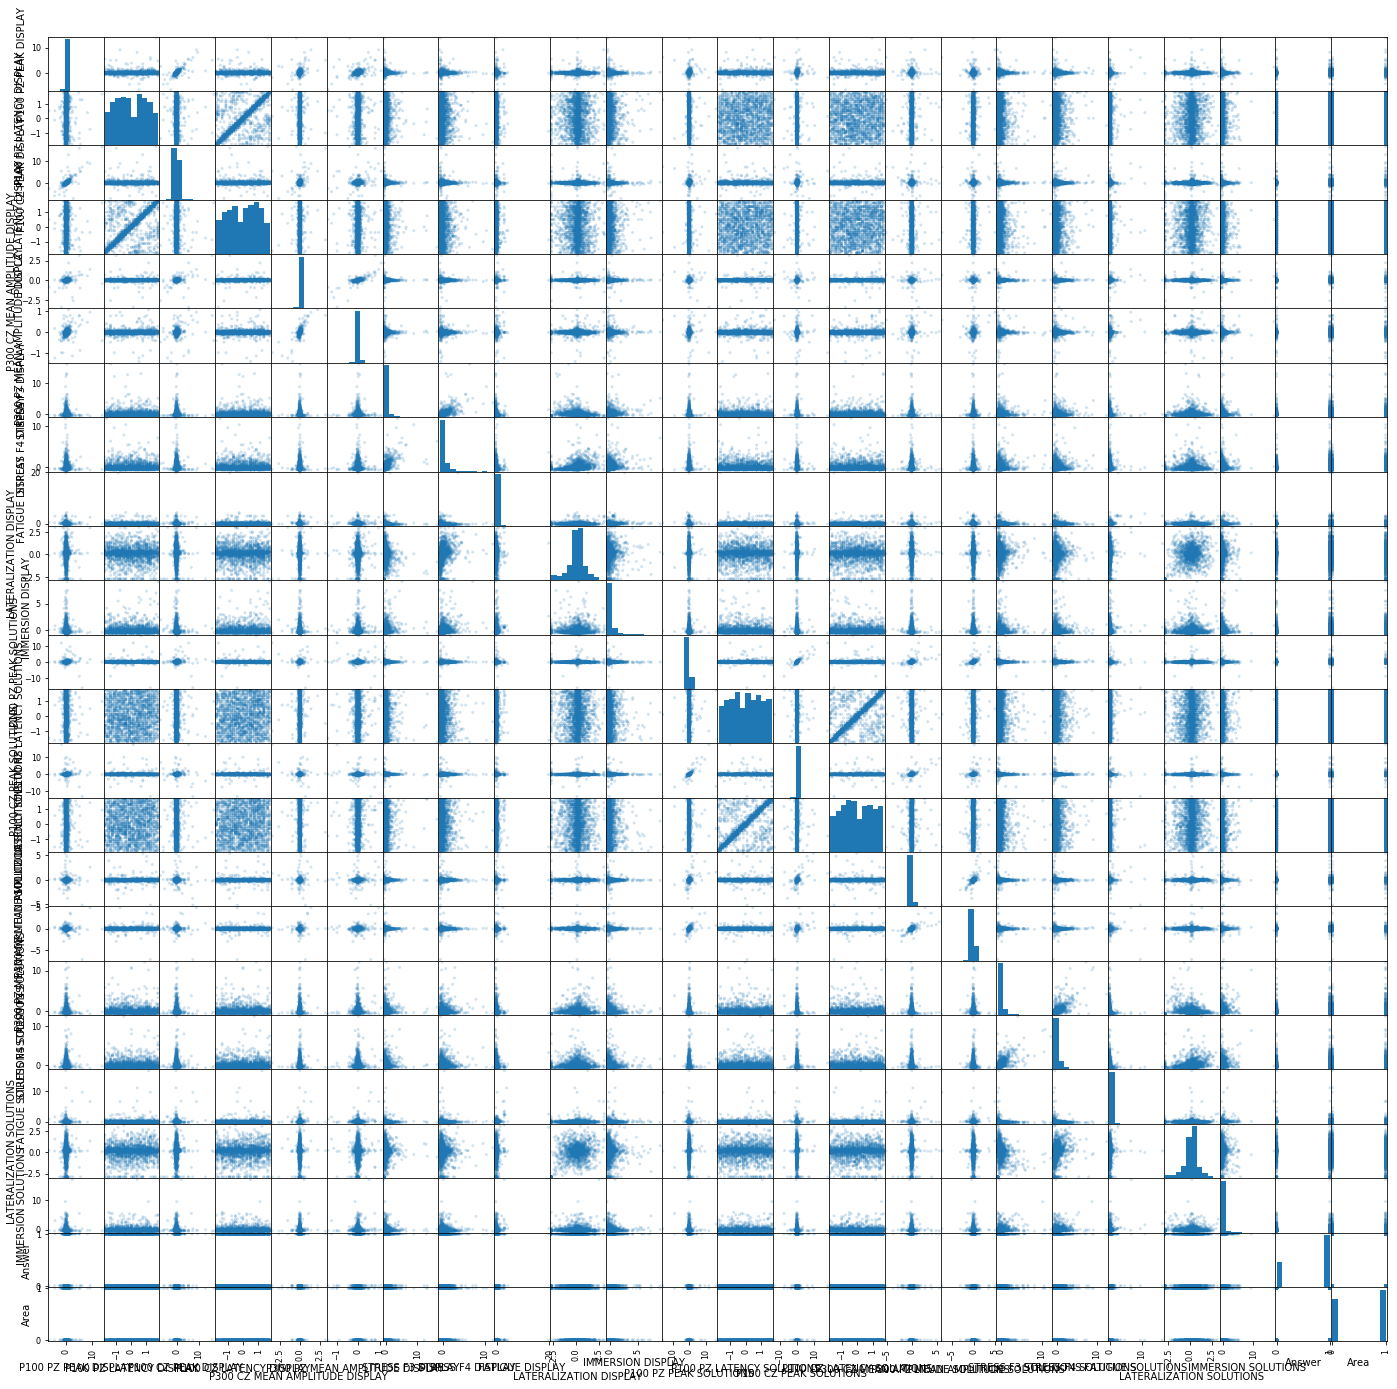
\includegraphics[width=2\linewidth]{featurecorrelation.png}
    \caption{Feature Correlations}
    \label{fig:feature}
\end{figure}

\end{document}
